\RequirePackage{xcolor}
\documentclass[a4]{sciposter}
\usepackage{multicol,subfig,amsmath} % columnas, figuras, ecuaciones
\usepackage{graphicx,url,hyperref,doi}
\hypersetup{hidelinks} 
\usepackage[spanish]{babel}   
\usepackage[utf8]{inputenc}
\usepackage[sort&compress,numbers]{natbib}
\usepackage[font=small,labelfont=bf]{caption}
\usepackage[bottom]{footmisc}

\usepackage{tikz} % diagramas
\tikzstyle{elem} = [draw, rectangle, thick, minimum height=2em, minimum width=2em]
\tikzstyle{line} = [draw, thick, -stealth, shorten >=1pt]

\setlength{\parskip}{3pt} % espacio entre parrafos
\renewcommand{\arraystretch}{1.5} % altura de renglones de cuadros

\leftlogo[1]{img/UANL.png}
\rightlogo[1]{img/FIME.png} 

\title{Mejora de algoritmo de\\reconocimiento de emociones}
\author{Cecilia Jael Aguilar Aranda$^\dagger$,\\Alexander Espronceda Gómez$^\ddagger$\\Satu Elisa Schaeffer$^\ast$}
\institute {$^\dagger$Ingeniería en Administración de Sistemas,  $^\ddagger$Ingeniería en Tecnologías de Software, \\Posgrado en Ingeniería de Sistemas$^\ast$}
\email{$^\dagger$cecilia.aguilarand@uanl.edu.mx, $^\ddagger$alexander.esproncedago@uanl.edu.mx}


\begin{document}
\conference{\raisebox{0mm}[0cm]{
\includegraphics[width=50mm]{img/qr-code-Poster.png}}
  \raisebox{0mm}[0cm]{
\includegraphics[width=50mm]{img/qr-code-Project.png}}
  \hfill
  \raisebox{20mm}[0cm]{\large Verano Científico 2021 --- Facultad de Ingeniería Mecánica y Eléctrica --- Universidad Autónoma de Nuevo León}
  \hfill
  \raisebox{10mm}[0cm]{
\includegraphics[width=100mm]{img/Provericyt-2021.png}}
  }

%\conference{\raisebox{8mm}{\large Verano Científico 2021 --- Facultad de Ingeniería Mecánica y Eléctrica --- Universidad Autónoma de Nuevo León}}

\maketitle

\begin{abstract}
En este proyecto se busca incrementar el funcionamiento de un algoritmo de análisis de sentimiento en base a texto utilizando redes neuronales. Esto conlleva realizar modificaciones al código, aí como el aumento del dataset con el que se trabaja. El objetivo es realizar un chatbot capaz de reconocer patrones, determinar el sentimeinto mostrado por el usuario y actuar acorde a ello.
\end{abstract}

\begin{multicols}{3} 

\section{Introducción}
El análisis de sentimiento se refiere a la aplicación de procesamiento de lenguaje natural, linguística computacional y análisis de texto para identificar la emoción del autor. \citep{definition}. En el presente documento se considera \textit{Análisis de sentimiento} y \textit{Reconocimiento de emociones} como un mismo concepto.

El objetivo principal de este proyecto es llevar a cabo diversos procesos que ayuden a que un algoritmo de análisis de sentimiento por medio de texto tenga un porcentaje de acierto más alto. Esto se logrará mediante búsqueda, análisis y filtrado de datos relevantes, así como también la actualización del algoritmo que está siendo utilizado actualmente.

\section{Antecedentes}

El algoritmo de análisis de sentimiento por medio de texto que se utiliza en este proyecto le corresponde a Alexander Espronceda Gómez, quien actualmente está escribiendo una tesis al respecto \citep{chatbot}. Por lo tanto, este proyecto sólamente se enfoca en el mejoramiento de éste, y no en el proceso completo.
\begin{figure}
	\centering
	\captionsetup{type=figure}
	\setcounter{figure}{0}
	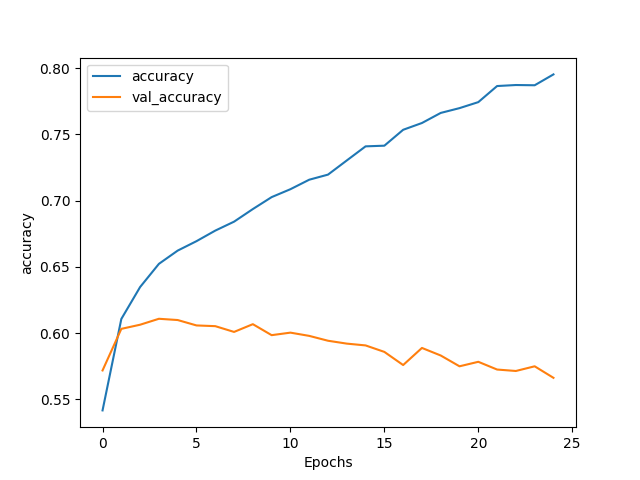
\includegraphics[scale=1.3]{img/Accuracy 2020-05_nofilter}
	\caption{Gráfica representativa del porcentaje de acierto del algoritmo, antes de aplicársele alguna mejora}
	
\end{figure}

\section{Estado de arte}

En la actualidad existen muchos algoritmos complejos de análisis de sentimiento que funcionan sin necesidad de introducirle tantos datos, tales como GPT-3 (Generative Pre-trained Transformer 3). En donde gracias a su uso eficiente de transformadores y también gracias a que ha sido entrenado extensamente con datasets enormes (por ejemplo: Wikipedia Corpus, Common Crawl, WebText2, entre otros), no hay necesidad de encontrar datos tan especificos para entrenarlos \citep{gpt3}.

Las opiniones son simples de entender para los humanos, pero, según \citet{liu}, para una computadora es necesario una noción con los siguientes elementos:

%\begin{itemize}
%    \item \textit{Objetivo} de la opinion: Entidades y sus características.
%    \item \textit{Sentimientos}: Positivos, negativos o neutrales
%    \item \textit{Poseedor} de la opinión
%    \item \textit{Tiempo} en el que las opiniones son expresadas.
%\end{itemize}

%También existen problemas relacionados al procesamiento de lenguaje natural (NLP). \citet{Dale} considera las siguientes las etapas del análisis de NLP:
%\begin{itemize}
%    \item \textit{Tokenización}: Convertir caracteres en palabras, símbolos u otros elementos llamados "tokens".
%    \item \textit{Análisis léxico}: Genera léxico y aplica etiquetas a los tokens.
%    \item \textit{Análisis sintáctico}: Proveer una estructura para cada oración.
%    \item \textit{Análisis semántico}: Encuentra el significado literal.
%    \item \textit{Análisis pragmático}: Determina el significado según el contexto.
%\end{itemize}

La gran diferencia entre el algoritmo propuesto en este proyecto y algo más elaborado como lo es GPT-3, es el hecho de que este último no funciona localmente, sino que en realidad es una API por la cual tienes que pagar para poder usar, además de que OpenAI tiene completo control y regulación de los usos de su algoritmo \citep{openai}. 

Lo que se intenta hacer al momento de utilizar TensorFlow es darle el control completo al usuario en caso de que quiera darle sesgo a los datos o que lo adapte a las necesidades que tenga, sin necesidad de que pase a ser una caja negra. Éste proceso es bastente complicado y probablemente no se alcanzará el grado de porcentaje de acierto con el que cuenta GPT-3, pero se espera que sea lo suficiente como para poder ser una alternativa open-source viable.



\section{Solución propuesta}
La implementación se hizo en Python 3.7 \citep{python}, además de otras herramientas relacionadas con redes neuronales como Tensorflow 2.0.0 \citep{tensorflow}.


\paragraph{Metodología}
Se comienza por una búsqueda de datasets, utilizándose la librería NLTK \citep{nltk} para filtrar palabras que no aportan mucho significado al texto.

Se considera mejor un enfoque generalista debido a que las diferentes etiquetas de sentimiento a analizar no estaban distribuidas de manera uniforme; por lo que los datos se clasifican únicamente en \textit{"Bueno"},\textit{"Neutral"} y \textit{"Malo"}.

Se utiliza un algoritmo bidireccional STM con una activación de softmax de última capa. El léxico está limitado a 5000 elementos, y el largo máximo de cualquier frase después de ser filtrada es de 30 caracteres.

Ya después de ser actualizado, el dataset utilizado cuenta con alrededor de 60,000 tweets filtrados y clasificados.

Durante la fase de entrenamiento, se utilizaron 25 epochs con un 75\% del dataset en un orden arbitrario, usando el 25\% restante como validación.

\begin{figure}
	\centering
	\captionsetup{type=figure}
	\setcounter{figure}{1}
	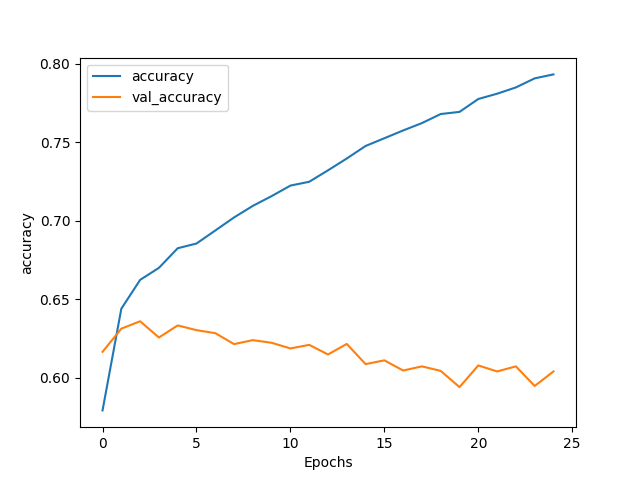
\includegraphics[scale=1.3]{img/Accuracy 2021-07.png}
	\caption{Gráfica representativa del porcentaje de acierto del algoritmo, después de aplicársele las mejoras propuestas}	
\end{figure}

\section{Experimentos}

Para determinar que este enfoque iba a funcionar, lo que hicimos fue correr varias veces el algoritmo con diferentes parámetros dentro de él, identificando áreas de oportunidad en donde podrían ir mejoras, y finalmente comparando reultados.

\begin{figure}
	\captionsetup{type=figure}
	\setcounter{figure}{2}
	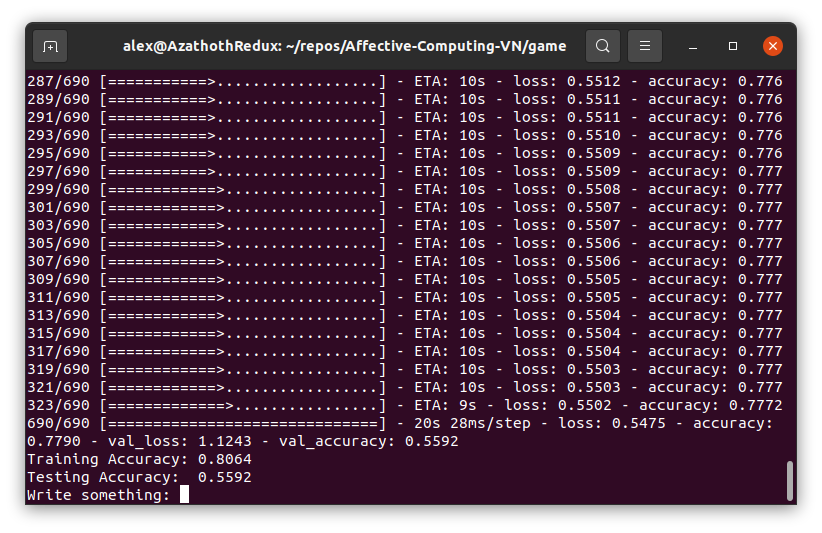
\includegraphics[scale=0.6]{img/Test 2021-05.png}
	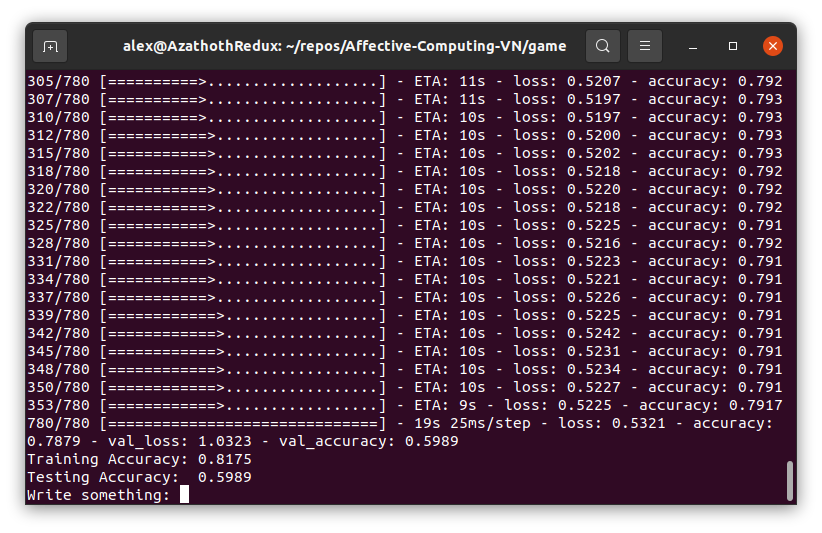
\includegraphics[scale=0.6]{img/Test 2021-07.png}
	\caption{Parámetros antes y después de la mejora}
\end{figure}

\begin{table}
\setcounter{table}{0} % por culpa de sciposter
\captionsetup{type=table} % por culpa de sciposter
\caption{Resultados de los experimentos antes y después de aplicarse la mejora}
\label{data}
\begin{center}
\scalebox{0.9}{\begin{tabular}{|r|c|l|}
    \hline
         \multicolumn{1}{|c|}{}
         & \multicolumn{1}{|c|}{\rotatebox{90}{\bf Precisión de entrenamiento }}
         & \multicolumn{1}{|c|}{\rotatebox{90}{\bf Precisión de testeo\phantom{m}}} \\
         \hline
         \bf{Antes} & 80.64\% & 55.92\% \\
         \hline
         \bf{Después} & 81.75\% & 59.89\% \\
        \hline
    \end{tabular}}
\end{center}
\end{table}

\section{Conclusiones}

Se ha logrado un aumento en la precisión de reconocimiento de emociones, se espera realizar más modificaciones para mejorar el algoritmo y en un futuro implementarlo para su uso.

\paragraph{Agradecimientos}

{\small El primer autor agradece a PROVERICYT al dar la oportunidad de participar en el Verano de Investigación Científica y Tecnológica 2021 y proporcionar una beca.
El póster se preparó con \url{https://www.overleaf.com/}.}
\end{multicols}

\bibliography{poster}
\bibliographystyle{unsrtnat}



\end{document}